% -------------------------------------------------
% - The same paper in IEEE two column format as
% - required by RuleML 2006
% -------------------------------------------------

\documentclass[10pt,twocolumn]{article}
\usepackage{latex8}
\usepackage{times}

\usepackage{graphicx}
\usepackage{epsfig}
\usepackage{xspace}
\usepackage{amssymb}
\usepackage{listings}
\usepackage{url}

\newcommand{\sgr}[1]{\textbf{sgr: {#1}}}
\newcommand{\wsml}[1]{\begin{scriptsize}{\sf {\bf #1}}\end{scriptsize}}

% WSML language keywords; and general syntax (for inline usage)
\newcommand{\synkw}[1]{\textsf{\scriptsize \textbf{#1}}}
\newcommand{\syn}[1]{\textsf{\scriptsize #1}}


\begin{document}

%%%%%%%%%%%%%%%%%%%%%%%%%%%%%%%%%%%%%%%%%%%%%%
%wsmo listings
\lstdefinelanguage{MOF}{
  alsodigit=-,%
  morekeywords={Class,type,multiplicity,single-valued,sub-Class},
  sensitive=true
}

\lstdefinestyle{mof}{
 language=MOF,
 basicstyle=\scriptsize\sffamily,
 keywordstyle=\bfseries,
 showstringspaces=false,
 flexiblecolumns=true,
 frame=tb,
 xleftmargin=15pt,
 xrightmargin=15pt,
}

%wsml listing
\lstdefinelanguage{WSML}{
  morekeywords={wsmlVariant,namespace,nonFunctionalProperties,endNonFunctionalProperties,importsOntology,
    usesMediator,ontology,goal,ooMediator,ggMediator,wgMediator,wwMediator,webService,concept,
    subConceptOf,ofType,impliesType,transitive,symmetric,inverseOf,reflexive,relation,subRelationOf,
    function,instance,relationInstance,memberOf,hasValue,axiom,definedBy,source,target,useService,
    capability,precondition,postcondition,assumption,effect,interface,choreography,orchestration,
    exists, forAll, implies, impliedBy, equivalent},
  sensitive=true,
  morestring=[b]",morestring=[d]�,
  morecomment=[s]{/*}{*/},
}

\lstdefinestyle{wsml}{
 language=WSML,
 basicstyle=\scriptsize\sffamily,
 keywordstyle=\bfseries,
 showstringspaces=false,
 mathescape=true,
 flexiblecolumns=true,
 frame=tb,
 xleftmargin=15pt,
 xrightmargin=15pt,
}


\lstdefinestyle{xml}{
 language=XML,
 basicstyle=\scriptsize\sffamily,
 keywordstyle=\bfseries,
 showstringspaces=false,
 mathescape=true,
 frame=tb,
 flexiblecolumns=true,
 xleftmargin=15pt,
 xrightmargin=15pt,
}


\title{A Reasoning Framework for Rule-Based WSML}

\author{Stephan Grimm$^1$, Uwe Keller$^2$, Holger Lausen$^2$ and G\'abor Nagyp\'al$^1$\\
\normalsize $^1$FZI Research Center for Information
Technologies at the University of Karlsruhe, Karlsruhe, Germany\\
\normalsize \sf $\{$grimm,nagypal$\}$@fzi.de\\[1mm]
\normalsize $^2$ Digital Enterprise Research Institute (DERI),
 University of Innsbruck, Austria\\ \normalsize \sf {$\{$uwe.keller,holger.lausen$\}$@deri.org} }

\maketitle

{\small

\begin{abstract}
%The use of ontology languages for semantically annotating Web
%Services demands for reasoning support in order to facilitate
%tasks like automated discovery or composition of services based on
%semantic descriptions of their functionality.
WSML is an ontology language specifically tailored to annotate Web
Services, and part of its semantics adheres to the rule-based
knowledge representation paradigm of logic programming. We present a
framework to support reasoning with rule-based WSML language
variants based on existing Datalog inference engines. Therein, the
WSML reasoning tasks of knowledge base satisfiability and instance
retrieval are implemented through a language mapping to Datalog
rules and Datalog querying. Part of the WSML semantics is realized
by a fixed set of rules that form meta-level axioms. Furthermore,
the framework exhibits some debugging functionality that allows for
identifying violated constraints and for pointing out involved
instances and problem types. Its highly modular architecture
facilitates easy extensibility towards other language variants and
additional features. The available implementation of the framework
provides the first reasoners for the WSML language.

\end{abstract}

\section{Motivation\label{sec:motivation}}
-- motivate the provision of reasoning support for (rule-based) WSML based on existing inference engines \\
-- -- in SWS, reasoning support for the ontology languages used is needed to perform e.g. matchmaking or type subsumption \\
-- -- a relatively new ontology language specific for SWS is WSML, which has variants following the  rule-based KR paradigm \\
-- -- we present a framework for reasoning with rule-based WSML \\
-- -- it bases on a semantics-preserving translation of WSML to datalog and thus builds on existing datalog inference engines \\
-- -- -- instead of directly mapping WSML to datalog, it realises the preserving of the WSML semantics by special meta-level predicates and axioms which build a vocabulary for reproducing the WSML language constructs in datalog \\
-- -- -- the WSML reasoning tasks can be performed by datalog querying \\
-- -- -- it supports debugging features for identifying violated constraints together with the involved ontological entities \\
-- -- it is implemented and can be readily used to reason with WSML ontologies; it is the first implementation of this kind \\
-- -- it is being developed within and partly funded by the DIP project where it is applied to SWS discovery and to support domain modelling in various use cases \\

In the Semantic Web, recently Web Services are annotated by
semantic descriptions of their functionality in order to
facilitate tasks like automated discovery or composition of
services. Such semantic annotation is formulated using ontology
languages with underlying logical formalisms. The matching of
semantic annotation for discovery or the checking of type
compatibility for composition requires reasoning support for these
languages. A relatively new ontology language specifically
tailored for the description of Web Services is WSML (Web Service
Modeling Language) \cite{wsml}, which comes in variants that
follow the rule-based knowledge representation paradigm of logic
programming \cite{}.

We present a framework for reasoning with rule-based WSML variants
that builds on existing infrastructure for inferencing in
rule-based formalisms. The framework bases on a
semantics-preserving syntactic transformation of WSML ontologies
to Datalog programs. Instead of directly mapping WSML entities,
i.e.\ concepts, instances, attributes, to datalog predicates and
constants, we use special meta-level predicates and axioms which
form a vocabulary on reified entities for reproducing the WSML
language constructs in the Datalog formalism, which facilitates
metamodelling features. The WSML reasoning tasks of checking
knowledge base satisfiability and of instance retrieval can then
be performed by means of Datalog querying applied on a transformed
ontology. Thus, the framework directly build on top of existing
Datalog inference engines. Besides these standard reasoning tasks,
the framework provides debugging features that support an ontology
engineer in the task of ontology development: the engineer is
pointed out to violated constraints together with some details on
the ontological entities that cause the violation. Such a feature
helps to improve the error reporting in situations of erroneous
modelling.

The framework is

\section{Reasoning in the WSML Language\label{sec:wsml}}
-- give an overview of the WSML language; focus on semantics of rule-based variants (also show how syntax looks like, e.g. by an example) \\
-- focus on the ontology language part of WSML (only briefly mention WS-specific parts) and sketch its features, such as constraints, datatypes, conceptual modelling + axiomatic formulations, ... \\
-- describe the reasoning tasks in WSML, i.e. KB satisfiability and entailment \\
-- relate language features and reasoning, e.g. constraints and satisfiability, to emphasise the close connection of these features to reasoning \\

The Web Service Modeling Language (WSML) is a language for the
specification of different aspects of Semantic Web Services. It
provides a formal language for the Web Service Modeling Ontology
WSMO which is based on well-known logical formalisms, specifying one
coherent language framework for the semantic description of Web
Services, starting from the intersection of Datalog and the
Description Logic $\mathcal{SHIQ}$. This core language is extended
in the directions of Description Logics and Logic Programming in a
principled manner with strict layering. WSML distinguishes between
conceptual and logical modeling in order to support users who are
not familiar with formal logic, while not restricting the expressive
power of the language  for the expert user. IRIs play a central role
in WSML as identifiers. Furthermore, WSML defines XML and RDF
serializations for inter-operation over the Semantic Web.

The Web Service Modeling Language WSML takes into account all
aspects of Web Service description identified by WSMO, i.e. Web
services, goals, mediators and ontologies. WSML comprises different
formalisms in order to investigate their applicability to the
description of SWS. It would have been too restrictive to base our
effort on existing language recommendations such as OWL
\cite{Dean+Schreiber-OntoLangRefe:04}. A concrete goal in our
development of WSML is to investigate the usage of different
formalisms, most notably Description Logics and Logic Programming,
in the context of Ontologies and Web services. Within this paper we
furthermore focus only on the Ontology part of WSML. Note that we
expect that reasoning tasks with the other elements of WSMO, e.g.
the over capabilities is expected to be reducible to reasoning tasks
within ontologies.

WSML makes a clear distinction between the modeling of the different
conceptual elements on the one hand and the specification of complex
logical definitions on the other. To this end, the WSML syntax is
split into two parts: the conceptual syntax and logical expression
syntax. The conceptual syntax was developed from the user
perspective, and is independent from the particular underlying
logic; it shields the user from the peculiarities of the underlying
logic. Having such a conceptual syntax allows for easy adoption of
the language, since it allows for an intuitive understanding of the
language for people not familiar with logical languages. In case the
full power of the underlying logic is required, the logical
expression syntax can be used. There are several entry points for
logical expressions in the conceptual syntax, namely, axioms in
ontologies and capability descriptions in Goals and Web Services.

\subsection{Conceptual Syntax}
\label{sec:conceptual-syntax}

The WSML conceptual syntax for ontologies allows for the modeling of
concepts, instances, relations and relation instances. Additionally,
an ontology may have non-functional properties and may import other
ontologies. We start the description of WSML ontologies with an
example which demonstrates the elements of an ontology in Listing
\ref{lst:wsml-ontology-example}, and detail the elements below.

\begin{lstlisting}[label=lst:wsml-ontology-example,style=wsml,caption={An
    Example WSML Ontology}]
wsmlVariant _"http://www.wsmo.org/wsml/wsml-syntax/wsml-flight"
namespace {_"http://example.org/bookOntology#",
        dc _"http://purl.org/dc/elements/1.1/"}
ontology _"http://example.org/bookOntology"
  nonFunctionalProperties
    dc#title hasValue "Example Book ontology"
    dc#description hasValue "Example ontology about books and shopping carts"
  endNonFunctionalProperties
    concept book
        title ofType _string
        hasAuthor ofType author
    concept author subConceptOf person
        authorOf inverseOf(hasAuthor) ofType book
    concept cart
      nonFunctionalProperties
        dc#description hasValue "A shopping cart has exactly one id
          and zero or more items, which are books."
      endNonFunctionalProperties
        id ofType (1) _string
        items ofType book
    instance crimeAndPunishment memberOf book
        title hasValue "Crime and Punishment"
        hasAuthor hasValue dostoyevsky

    relation authorship(impliesType author, impliesType document)
      nonFunctionalProperties
        dc#relation hasValue authorshipFromAuthor
      endNonFunctionalProperties

    axiom authorshipFromAuthor
      definedBy
        authorship(?x,?y) :- ?x[authorOf hasValue ?y] memberOf author.
\end{lstlisting}

\paragraph{Concepts}
The notion of concepts (sometimes also called `classes') plays a
central role in ontologies. Concepts form the basic terminology of
the domain of discourse. A concept may have instances and may have a
number of attributes associated with it. The non-functional
properties, as well as the attribute definitions, are grouped
together in one frame, as can be seen from the example concept
\syn{book} in Listing \ref{lst:wsml-ontology-example}.

Attribute definitions can take two forms, namely \emph{constraining}
(using \synkw{ofType}) and \emph{inferring} (using
\synkw{impliesType}) attribute definitions\footnote{The distinction
  between inferring and constraining attribute definitions is
  explained in more detail in \cite[Section
  2]{Bruijn+PolleresETAL-:05}}. Constraining attribute definitions
define a typing constraint on the values for this attribute, similar
to integrity constraints in Databases; inferring attribute
definitions imply that the type of the values for the attribute is
inferred from the attribute definition, similar to range
restrictions on properties in
RDFS~\cite{Brickley+Guha-VocaDescLang:03} and
OWL~\cite{Dean+Schreiber-OntoLangRefe:04}.  Each attribute
definition may have a number of features associated with it, namely,
transitivity, symmetry, reflexivity, and the inverse of an
attribute, as well as minimal and maximal cardinality constraints.

Constraining attribute definitions, as well as cardinality
constraints, require closed-world reasoning and are thus not allowed
in WSML-Core and WSML-DL. As opposed to features of roles in
Description Logics, attribute features such as transitivity,
symmetry, reflexivity and inverse attributes are local to a concept
in WSML. Thus, none of these features may be used in WSML-Core and
WSML-DL. For a motivation on the use of constraining attributes, see
\cite{Bruijn+PolleresETAL-:05}.

\paragraph{Relations}
Relations in WSML can have an arbitrary arity, may be organized in a
hierarchy using \synkw{subRelationOf} and the parameters may be
typed using parameter type definitions of the form
(\syn{\synkw{ofType}
  $type$} ) and (\syn{\synkw{impliesType} $type$}), where $type$ is a
concept identifier. The usage of \synkw{ofType} and
\synkw{impliesType} correspond with the usage in attribute
definitions. Namely, parameter definitions with the \synkw{ofType}
keyword are used to check the type of parameter values, whereas
parameter definitions with the \synkw{impliesType} keyword are used
to infer concept membership of parameter values.

The allowed arity of the relation may be constrained by the
underlying logic of the WSML language variant. WSML-Core and WSML-DL
allow only binary relations and, similar to attribute definitions,
they allow only parameter typing using the keyword
\synkw{impliesType}.


\paragraph{Instances}
A concept may have a number of instances associated with it.
Instances explicitly specified in an ontology are those which are
shared as part of the ontology. However, most instance data exists
outside the ontology in private databases. WSML does not prescribe
how to connect such a database to an ontology, since different
organizations will use the same ontology to query different
databases and such corporate databases are typically not shared.

An instance may be member of zero or more concepts and may have a
number of attribute values associated with it, see for example the
instance \syn{crimeAndPunishment} in Listing
\ref{lst:wsml-ontology-example}. Note that the specification of
concept membership is optional and the attributes used in the
instance specification do not necessarily have to occur in the
associated concept definition. Consequently, WSML instances can be
used to represent semi-structured data, since without concept
membership and constraints on the use of attributes, instances form
a directed labelled graph. Because of this possibility to capture
semi-structured data, most RDF graphs can be represented as WSML
instance data, and vice versa.


\paragraph{Axioms} Axioms provide a means to add arbitrary logical
expressions to an ontology. Such logical expressions can be used to
refine concept or relation definitions in the ontology, but also to
add arbitrary axiomatic domain knowledge or express constraints. The
axiom \syn{authorshipFromAuthor} in Listing
\ref{lst:wsml-ontology-example} states that the relation
\syn{authorship} exists between any author and any book of which he
is an author; consequently, $\langle \syn{dostoyesksy},
\syn{crimeAndPunishment} \rangle$ is in the relation
\syn{authorship}. Logical expressions are explained in more detail
in Section~\ref{sec:log-expr-syntax}.

\subsection{Logical Expression Syntax}
\label{sec:log-expr-syntax}

We will first explain the general logical expression syntax, which
encompasses all WSML variants, and then describe the restrictions on
this general syntax for each of the variants. The general logical
expression syntax for WSML has a First-Order Logic style, in the
sense that it has constants, function symbols, variables, predicates
and the usual logical connectives. Furthermore, WSML has F-Logic
\cite{Kifer+LausenETAL-LogiFounObjeFram:95} based extensions in
order to model concepts, attributes, attribute definitions, and
subconcept and concept membership relationships. Finally, WSML has a
number of connectives to facilitate the Logic Programming based
variants, namely default negation (negation-as-failure),
LP-implication (which differs from classical implication) and
database-style integrity constraints.

Variables in WSML start with a question mark, followed by an
arbitrary number of alphanumeric characters, e.g., \syn{?x},
\syn{?name}, \syn{?123}. Free variables in WSML (i.e., variables
which are not explicitly quantified), are implicitly universally
quantified outside of the formula (i.e., the logical expression in
which the variable occurs is the scope of quantification), unless
indicated otherwise, through the \synkw{sharedVariables} construct
(see the previous Section).

Terms are either identifiers, variables, or constructed terms. An
atom is, as usual, a predicate symbol with a number of terms as
arguments. Besides the usual atoms, WSML has a special kind of
atoms, called \emph{molecules}, which are used to capture
information about concepts, instances, attributes and attribute
values. The are two types of molecules, analogous to F-Logic:

\begin{itemize}
\item An \emph{isa} molecule is a concept membership molecule of
  the form \syn{\emph{A} \synkw{memberOf} \emph{B}} or a subconcept
  molecule of the form \syn{\emph{A} \synkw{subConceptOf} \emph{B}}
  with \syn{\emph{A}} and \syn{\emph{B}} arbitrary terms

\item An \emph{object} molecule is an attribute value expressions
  of the form \syn{\emph{A}[\emph{B} \synkw{hasValue} \emph{C}]}, a
  constraining attribute signature expression of the form
  \syn{\emph{A}[\emph{B} \synkw{ofType} \emph{C}]}, or an inferring attribute signature expression of the form
  \syn{\emph{A}[\emph{B} \synkw{ofType} \emph{C}]}, with
  \syn{\emph{A,B,C}} arbitrary terms
\end{itemize}

WSML has the usual first-order connectives: the unary negation
operator \synkw{neg}, and the binary operators for conjunction
\synkw{and}, disjunction \synkw{or}, right implication
\synkw{implies}, left implication \synkw{impliedBy}, and dual
implication \synkw{equivalent}. Variables may be universally
quantified using \synkw{forall} or existentially quantified using
\synkw{exists}. First-order formulae are obtained by combining atoms
using the mentioned connectives in the usual way. The following are
examples of First-Order formulae in WSML:

\begin{lstlisting}[style=wsml, frame=none]
//every person has a father
forall ?x (?x memberOf Person implies exists ?y (?x[father hasValue
?y])).
//john is member of a class which has some attribute called 'name'
exists ?x,?y (john memberOf ?x and ?x[name ofType ?y]).
\end{lstlisting}

Apart from First-Order formulae, WSML allows the use of the
negation-as-failure symbol \synkw{naf} on atoms, the special Logic
Programming implication symbol \synkw{:-} and the integrity
constraint symbol \synkw{!-}. A logic programming rule consists of a
\emph{head} and a \emph{body}, separated by the \synkw{:-} symbol.
An integrity constraint consists of the symbol \synkw{!-} followed
by a rule body. Negation-as-failure \synkw{naf} is only allowed to
occur in the body of a Logic Programming rule or an integrity
constraint. The further use of logical connectives in Logic
Programming rules is restricted. The following logical connectives
are allowed in the head of a rule: \synkw{and}, \synkw{implies},
\synkw{impliedBy}, and \synkw{equivalent}. The following connectives
are allowed in the body of a rule (or constraint): \synkw{and},
\synkw{or}, and \synkw{naf}. The following are examples of LP rules
and database constraints:

\begin{lstlisting}[style=wsml, frame=none]
//every person has a father
?x[father hasValue f(?y)] :- ?x memberOf Person.
//Man and Woman are disjoint
!- ?x memberOf Man and ?x memberOf Woman.
//in case a person is not involved in a marriage, the person is a bachelor
?x memberOf Bachelor :- ?x memberOf Person and naf
Marriage(?x,?y,?z).
\end{lstlisting}

\subsection{Particularities of the WSML Variants}

Each of the WSML variants defines a number of restrictions on the
logical expression syntax. For example, LP rules and constraints are
not allowed in WSML-Core and WSML-DL. Table \ref{table:wsml-matrix}
presents a number of language features and indicates in which
variant the feature can occur.

\begin{table}[ht]
\center
\begin{tabular}{|l|c|c|c|c|c|}
    \hline
Feature             & Core  & DL    & Flight    & Rule  & Full \\
    \hline
Classical Negation (\synkw{neg})
                    & -     & X     & -         & -     & X \\
Existential Quantification
                    & -     & X     & -         & -     & X \\
(Head) Disjunction
                    & -     & X     & -         & -     & X \\
$n$-ary relations
                    & -     & -     & X         & X     & X \\
Meta Modeling
                    & -     & -     & X         & X     & X \\
Default Negation (\synkw{naf})
                    & -     & -     & X         & X     & X \\
LP implication
                    & -     & -     & X         & X     & X \\
Integrity Constraints
                    & -     & -     & X         & X     & X \\
Function Symbols
                    & -     & -     & -         & X     & X \\
Unsafe Rules
                    & -     & -     & -         & X     & X \\
    \hline
\end{tabular}
\caption{WSML Variants and Feature Matrix} \label{table:wsml-matrix}
\end{table}

\begin{itemize}
\item \emph{WSML-Core}
allows only first-order formulae which can be translated to the DLP
subset of $\mathcal{SHIQ}(\mathbf{D)}$
\cite{Grosof+HorrocksETAL-DescLogiProg:03}. This subset is very
close to the 2-variable fragment of First-Order Logic, restricted to
Horn logic. Although WSML-Core might appear in the Table
\ref{table:wsml-matrix} featureless, it captures most of the
conceptual model of WSML, but has only limited expressiveness within
the logical expressions.

\item \emph{WSML-DL}
allows first-order formulae which can be translated to
$\mathcal{SHIQ}(\mathbf{D)}$. This subset is very close to the
2-variable fragment of First-Order Logic. Thus, WSML DL allows
classical negation, and disjunction and existential quantification
in the heads of implications.

\item \emph{WSML-Flight}
extends the set of formulae allowed in WSML-Core by allowing
variables in place of instance, concept and attribute identifiers
and by allowing relations of arbitrary arity. In fact, any such
formula is allowed in the head of a WSML-Flight rule. The body of a
WSML-Flight rule allows conjunction, disjunction and default
negation. The head and body are separated by the LP implication
symbol.

WSML-Flight additionally allows meta-modeling (e.g.,
classes-as-instances) and reasoning over the signature, because
variables are allowed to occur in place of concept and attribute
names.

\item \emph{WSML-Rule}
extends WSML-Flight by allowing function symbols and unsafe rules,
i.e., variables which occur in the head or in a negative body
literal do not need to occur in a positive body literal.

\item \emph{WSML-Full}
The logical syntax of WSML-Full is equivalent to the general logical
expression syntax of WSML and allows the full expressiveness of all
other WSML variants.

\end{itemize}

The separation between conceptual and logical modeling allows for an
easy adoption by non-experts, since the conceptual syntax does not
require expert knowledge in logical modeling, whereas complex
logical expressions require more familiarity and training with the
language. Thus, WSML allows the modeling of different aspects
related to Web services on a conceptual level, while still offering
the full expressive power of the logic underlying the chosen WSML
variant. Part of the conceptual syntax for ontologies has an
equivalent in the logical syntax. This correspondence is used to
define the semantics of the conceptual syntax. Notice that, since
only parts of the conceptual syntax are mapped to the logical
syntax, only a part of the conceptual syntax has a semantics in the
logical language for ontologies. For example, non-functional
properties are not translated (hence, the name `non-functional').
The translation between the conceptual and logical syntax is
sketched in Table \ref{tab:conceptual-logical}.

\begin{table}[ht]
  \centering
\footnotesize{
  \begin{tabular}{l|l}
    \textbf{Conceptual} & \textbf{Logical} \\
\hline
    \begin{lstlisting}[style=wsml-table]
concept A subConcepOf B
    \end{lstlisting}
    &
    \begin{lstlisting}[style=wsml-table]
A subConceptOf B.
    \end{lstlisting}
    \\
    \begin{lstlisting}[style=wsml-table]
concept A
  B ofType (0 1) C
    \end{lstlisting}
    &
    \begin{lstlisting}[style=wsml-table]
A[B ofType C]. !- ?x memberOf A and
  ?x[B hasValue ?y, B hasValue ?z] and ?y != ?z.
    \end{lstlisting}\\
    \begin{lstlisting}[style=wsml-table]
concept A B ofType C
    \end{lstlisting}
    &
    \begin{lstlisting}[style=wsml-table]
A[B ofType C].
    \end{lstlisting}\\
    \begin{lstlisting}[style=wsml-table]
relation A/n subRelationOf B
    \end{lstlisting}
    &
    \begin{lstlisting}[style=wsml-table]
A(x$_1$,...,x$_n$) implies B(x$_1$,...,x$_n$)
    \end{lstlisting}\\
    \begin{lstlisting}[style=wsml-table]
instance A memberOf B
  C hasValue D
    \end{lstlisting}
    &
    \begin{lstlisting}[style=wsml-table]
A memberOf B. A[C hasValue D].
    \end{lstlisting}\\
    \hline
  \end{tabular}}

  \caption{Translating conceptual to logical
    syntax}\label{tab:conceptual-logical}
\end{table}

\newcommand{\smtxtit}[1]{\begin{scriptsize}\ensuremath{\textit{#1}}\end{scriptsize}}
\newcommand{\trans}[1]{\ensuremath{\tau_{#1}}\xspace}
\newcommand{\transtxt}[1]{\trans{\smtxtit{#1}}}
%\newcommand{\transmap}[3]{\ensuremath{\tau_{#1}^{{#2},{#3}}}\xspace}
%\newcommand{\transtxtmap}[3]{\transmap{\smtxtit{#1}}{#2}{#3}}
\def\LE{\ensuremath{\mathcal{L\!E}}\xspace}
\def\O{\ensuremath{\mathcal{O}}\xspace}
\def\P{\ensuremath{\mathcal{P}}\xspace}
\newcommand{\powset}[1]{\ensuremath{2^{#1}}\xspace}

\section{Realistion of WSML Reasoning through a Mapping to Datalog\label{sec:mapping}}
-- briefly sketch the idea of reasoning via rule based inferencing \\

The semantics of rule-based WSML is defined via a mapping to
datalog with (in)equality and integrity constraints. \sgr{probably
use a special denotation like $\textit{datalog}^{!=,IC}$, which
then has to be introduced in Section 2} Thus, the reasoning
framework performs various transformations to convert an original
ontology in WSML syntax into datalog rules. To maintain the
semantics of more complex WSML language constructs that cannot
directly be expressed in datalog, a fixed set of rules form the
meta-level axioms that realise part of the WSML semantics during
reasoning. Finally, the WSML reasoning tasks of knowledge base
satisfiability and instance retrieval are realised by datalog
querying via calls to an underlying datalog inference engine that
is fed with the rules produced during transformation together with
the meta-level axioms.

\subsection{Transformation of WSML into Datalog}
-- describe different transformation steps \\

The transformation of a WSML ontology to datalog rules forms a
pipeline of single transformation steps which are subsequently
applied, starting from the original ontology.

\paragraph{Axiomatization} -- In a first step, the transformation
\transtxt{axiom} is applied as a mapping $\O \mapsto \powset{\LE}$
from the set of all valid ontologies formulated in rule-based WSML
to the powerset of all logical expressions that conform to
rule-based WSML. \transtxt{axiom} converts all conceptual syntax
elements, such as concept and attribute definitions or cardinality
and type constraints, into appropriate logical expressions
according to \cite{wsml-spec}(Table 8.1). \sgr{give the complete
conversion table ??}

To give an example, the WSML fragment
\begin{quote}
\begin{lstlisting}[style=wsml]
concept C subConceptOf D
    r ofType (0 2) T
instance a memberOf C
    r hasValue b,c
\end{lstlisting}
\end{quote}
is translated by \transtxt{axiom} to the following logical
expressions.

\begin{quote}
\begin{lstlisting}[style=wsml]
C subConceptOf D.%
!- ?x memberOf C and ?x[r hasValue ?y] and naf ?y memberOf T.%
!- ?x memberOf C and ?x[r hasValue ?y1, r hasValue ?y2] and ?y1 != ?y2.%
a memberOf C.  a hasValue b,c.
\end{lstlisting}
\end{quote}

\paragraph{Normalization} -- The transformation \transtxt{norm} is
applied to normalize WSML logical expressions as a mapping
$\powset{\LE} \mapsto \powset{\LE}$. This normalization step
reduces the complexity of WSML logical expressions according to
\cite{wsml-spec}(Section 8.2) to make them better fit the simple
syntactic form of literals in datalog rules. This reduction
includes conversion to negation and disjunctive normal forms as
well as decomposition of complex WSML molecules (see
\cite{wsml-spec}).

\paragraph{Lloyd-Topor Transformation} -- The transformation
\transtxt{Lloyd-Topor} is applied as a mapping $\powset{\LE}
\mapsto \powset{\LE}$ to flatten the complex WSML logical
expressions, producing simple rules according to the Lloyd-Topor
transformations \cite{lloyd-topor} as follows.
\begin{center}
\begin{tabular}{|c|c|}
  \hline
  % after \\: \hline or \cline{col1-col2} \cline{col3-col4} ...
  \emph{original expression} & \emph{simplified rule(s)} \\
  \hline
  $H_1 \wedge H_2 \wedge \dots \wedge H_n \leftarrow B$ & $H_1 \leftarrow B , H_2 \leftarrow B , \dots , H_n \leftarrow B$ \\
  $H_1 \leftarrow H_2 \leftarrow B$ & $H_1 \leftarrow H_2 \wedge B$ \\
  $H \leftarrow B_1 \vee B_2 \vee \dots \vee B_n$ & $H \leftarrow B_1 , H \leftarrow B_2 , \dots , H \leftarrow B_n$ \\
  \hline
\end{tabular}
\end{center}

After this step, the resulting WSML expressions have the form of
proper datalog rules with a single head and conjunctive (possibly
negated) body literals.

\paragraph{Datalog Rule Generation} -- In a final step, the
transformation \transtxt{datalog} is applied as a mapping
$\powset{\LE} \mapsto \P$ from all valid logical expressions in
rule-based WSML to the set of all datalog programs, yielding
generic datalog rules that represent the content of the original
WSML ontology. In this generic datalog program, all remaining
WSML-specific language constructs, such as \wsml{subConceptOf} or
\wsml{ofType}, are replaced by special meta-level predicates for
which the semantics of the respective language construct is
encoded in meta-level axioms as described in a further subsection.
\begin{table}[b]\label{tab:LE2datalog}\centering
\begin{tabular}{|l|c|}
  \hline
  bla & bla \\
  \hline
\end{tabular}
\caption{Transformation from logical expressions in rule-based
WSML to datalog including meta-level predicates.}
\end{table}
Table \ref{tab:LE2datalog} shows the mapping from WSML logical
expressions to generic datalog including such meta-level
predicates.

Notice that the \wsml{memberOf} construct for instantiation is
also mapped to an appropriate meta-level predicate instead of
direct instantiation of the form $C(i)$, which is available in
datalog. This decision was taken in order to facilitate the
metamodelling capabilities of rule-based WSML, which allows an
entity to be both an instance and class at the same time.
\sgr{genauer darstellen f�r was welche metal-level Predikate
erzeugt werden!}

\bigskip

Ultimately, the basic transformation pipeline for converting a
rule-based WSML ontology into a datalog program is the following,
constituted by the single transformation steps introduced before.
\begin{displaymath}
    \tau = \transtxt{datalog} \circ \transtxt{Lloyd-Topor} \circ \transtxt{norm} \circ \transtxt{axiom}
\end{displaymath}
As a mapping $\O \mapsto \P$, this chaining of the single steps is
applied to a WSML ontology $O \in \O$ to yield a semantically
equivalent datalog program $\tau (O) = P \in \P$ when interpreted
with respect to the meta-level axioms discussed next.

\subsection{Realising WSML Semantics through Meta Axioms}
-- describe how a fixed set of rules implements (part of) the WSML semantics during reasoning \\

The mapping from WSML to datalog in the reasoning framework works
such that all WSMl-identifiable entities, namely concepts,
instances, attributes etc., are mapped to datalog instances.

\subsection{Mapping WSML Reasoning Tasks to Datalog Querying}
-- describe how to realise WSML satisfiability and entailment to datalog querying \\

\subsection{Realising Datatype Reasoning}
-- describe how reasoning with datatypes is realised

\def\transdebug{\transtxt{debug}}
\def\pvotype{\predicate{\predsubtxt{v\_otype}}}
\def\pvmincard{\predicate{\predsubtxt{v\_mincard}}}
\def\pvmaxcard{\predicate{\predsubtxt{v\_maxcard}}}
\def\pvuser{\predicate{\predsubtxt{v\_user}}}
\def\axiomid{\ensuremath{Ax_{I\!D}}}
\def\debugaxioms{\ensuremath{P_{\smtxtit{debug}}}\xspace}

\section{Debugging Support\label{sec:debugging}}
-- briefly motivate debugging for the ontology engineering process \\
-- -- during the process of ontology engineering, a modeller easily produces erroneous contradictory information, which he needs to get aware of \\
-- -- the source for contradictory information in rule-based WSML are primarily constraints \\
-- -- with plain datalog mechanisms, modellers only get aware of whether some constraint is violated, i.e. whether the empty clause is derived from $P_O$ indicating that the original ontology $O$ contains erroneous modelling; the modeller is not informed about the type of problem and why the problem occurs \\
-- -- our framework offers debugging features that allow for identifying violated constraints and involved WSML entities, which is achieved by replacing constraints by rules with special additional meta-level predicates in their head \\

\subsection{Identifying Constraint Violations}
-- describe the kind of debugging features the framework supports and what they allow for \\
-- -- in a WMSL ontology, constraints can be violated by the instance situation, making the ontology inconsistent \\
-- -- two things a of interest to the modeller when a constraint is violated: a) the type of constraint and the entities involved \\
-- -- $<$ give an example of a violated constraint to illustrate what information is relevant for the modeller in such a situation $>$ \\
-- -- in the different situations of violation of different types of constraints, different information is relevant for the modeller to repair the erroneous situation  \\
-- -- $<$ list different types of violations $>$ \\

\subparagraph{Attribute Type Violation} -- An attribute type
constraint of the form $C[a$ \wsml{ofType} $T]$ is violated in any
situation where an instance of the concept $C$ has value $V$ for
the attribute $a$ but where $V$ cannot be derived to belong to the
extension of the type $T$. Here, $T$ can be either a concept or a
datatype, while $V$ is then an instance or a data value,
accordingly. In such a situation, an ontology engineer is
particularly interested in the attribute value $V$ that caused the
constraint violation, together with the attribute $a$ and the
expected type $T$ which the value $V$ failed to adhere to.

\subparagraph{Minimum Cardinality Violation} -- A minimum
cardinality constraint, contained in a concept definition of the
form \wsml{concept} $C$ $a (n *)$, is violated in any situation
where the number of distinguished values of the attribute $a$ for
some instance $I$ of the concept $C$ is less than the specified
cardinality $n$. In such a situation, an ontology engineer is
particularly interested in the instance $I$ that failed to have a
sufficient number of attribute values, together with the actual
attribute $a$. (Information about how many values were missing can
be learned by querying the ontology separately.)

\subparagraph{Maximum Cardinality Violation} -- A maximum
cardinality constraint, contained in a concept definition of the
form \wsml{concept} $C$ $a (0 n)$, is violated in any situation
where the number of distinguished values of the attribute $a$ for
some instance $I$ of the concept $C$ exceeds the specified
cardinality $n$. Again, here an ontology engineer is particulary
interested in the instance $I$ for which the number of attribute
values has been exceeded, together the actual attribute $a$.

\subparagraph{User-Defined Constraint Violation} -- A user-defined
constraint, contained in an axiom definition of the form
\wsml{axiom} \axiomid \wsml{definedBy} $B.$, is violated in any
situation where the body $B$ of the constraint evaluates to true
for any instantiation of its free variables. In such a situation,
the information which helps an ontology engineer to repair an
erroneous situation is specific to the user-defined constraint
given by $B$ and cannot be specified in a generic manner. However,
a generic framework can at least identify the violated constraint
by pointing out the name \axiomid of the axiom.

\subsection{Debugging through Meta-Level Reasoning}
-- describe how these debugging features are realised via additional meta-level predicates an additional fixed set of rules \\
-- -- in our framework we realise the debugging features for identifying constraint violations together with involved entities by replacing constraints with rules \\
-- -- these rules have additional debugging-specific meta-level predicates in their heads which are instantiated when a constraint body evaluates to true; this way the debugging information is derived by datalog rules and can be queried for \\
-- -- the replacements of constraints is included in the transformation pipeline $\tau$ as an additional step \\
\begin{displaymath}
    \tau = \transdlog \circ \translt \circ \transnorm \circ \transdebug \circ \transax
\end{displaymath}
-- -- the additional transformation step $\transdebug$ is applied after conceptual syntax has been resolved, replacing constraints on the level of WSML logical expressions \\
-- -- the detailed constrained replacement performed by \transdebug can be seen from Table \ref{tab:debugging} \\
-- -- the body variables are supposed to match the appropriate form of constraint body; notice: the semantics of ofType is encoded in the meta-level axioms \mlaxioms, so ofType-constraints can't be as easily replaced but have to be generated by \transdebug \\
-- -- to maintain the constraint-semantics, some additional debugging-specific meta-level axioms, denoted by \debugaxioms, have to be included, which are shown in Table \ref{tab:debugging-axioms} \\
-- -- thus, the datalog program used for reasoning with the original WSML ontology turns to: \\
\begin{displaymath}
    P_O = \mlaxioms \cup \debugaxioms \cup \tau(O)
\end{displaymath}
-- -- then one can ask for occurrences of the different kinds of constraint violation by e.g. \\
\begin{displaymath}
    \{(a,T,I,V) : (P_O , ?\pvotype(a,T,I,V)) \rightarrow \top \}
\end{displaymath}
-- -- which asks for all occurrences of type violations by means of datalog querying mechanisms; if this set is empty then there is no problem concerning types \\

In our framework, we realize the debugging features for pointing
out constraint violations by replacing constraints with a special
kind of rules. Instead of deriving the empty clause as constraints
do, these rule derive information about occurrences of constraint
violations by instantiating debugging-specific meta-level
predicates with the entities involved in a violation. In this way,
information about constraint violations can be queried for by
means of datalog inferencing.

The replacement of constraints for debugging is included in the
transformation pipeline
\begin{displaymath}
    \tau = \transdlog \circ \translt \circ \transnorm \circ \transdebug \circ \transax
\end{displaymath}
where the additional transformation step \transdebug is applied
after the WSML conceptual syntax has been resolved, replacing
constraints on the level of WSML logical expressions. Table
\ref{tab:debugging} shows the detailed replacements performed by
\transdebug for the different kinds of constraints.

The two types of cardinality constraints with bodies $B_{mincard}$
and $B_{maxcard}$ are turned into rules by keeping the respective
body and including a head that instantiates one of the predicates
\pvmincard and \pvmaxcard to indicate the respective cardinality
violation. The body variables are supposed to syntactically match
the respective bodies for cardinality constraints produced by
\transax (Table \ref{tab:conceptual-logical}), in which the
arguments for these predicates, namely the involved attribute $a$
and instance $I$, occur. Similarly, a user-defined constraint is
turned into a rule by keeping the predefined body $B_{user}$ and
including a head that instantiates the predicate \pvuser to
indicate a user-defined violation. Since the body $B_{user}$ can
be an arbitrarily complex logical expression, the only argument of
this predicate is the identifier \axiomid of the axiom that
contains the  specification of the user-defined constraint.
Contrarily, constraints on attribute types are handled in a
different way because these constraints are not expanded during
the transformation \transax ; they are rather represented by WSML
\wsml{ofType} molecules for which the semantics is encoded in the
meta-level axioms \mlaxioms. In order to avoid the modification of
\mlaxioms in the reasoning framework, such molecules are expanded
by \transdebug, as shown in Table
\ref{tab:debugging}.\footnote{After this expansion of
\wsml{ofType} molecules, the respective axiom in \mlaxioms for
realising the semantics of attribute type constraints does not
apply anymore.}

To maintain the constraining semantics of the replaced
constraints, an additional set of meta-level axioms $\debugaxioms
\in \mathcal{P}$ is included for reasoning that derive the empty
clause for any occurrence of a constraint violation, as shown in
Table \ref{tab:debugging-axioms}. Including the debugging
features, the datalog program used to reason about the original
ontology then turns to
\begin{displaymath}
    P_O = \mlaxioms \cup \debugaxioms \cup \tau(O) \;\;\;.
\end{displaymath}
Occurrences of constraint violations can be recognized by querying
$P_O$ for instantiations of the various debugging-specific
meta-level predicates \pvotype, \pvmincard, \pvmaxcard and
\pvuser. For example, the set
\begin{displaymath}
    \{(a,T,I,V) : (P_O , ?\pvotype(a,T,I,V)) \rightarrow \top \}
\end{displaymath}
contains tuples for all occurrences of attribute type violations
in $P_O$, identifying the respective attribute $a$, expected type
$T$, involved instance $I$ and violating value $V$ for each. This
set is empty if there are no types violated in $P_O$.


\begin{table}[tb]\label{tab:debugging}\centering
\begin{footnotesize}
\begin{tabular}{|l|l|}
  \hline
  \rule{0cm}{3.2mm} {\normalsize \emph{Constraint}} & {\normalsize \emph{Rule}} \\
  \hline
  $\transdebug($\wsml{\cstr}$B_{mincard}.)$ & $\pvmincard(a,I)$\wsml{\lprl}$B_{mincard}.$ \\
  $\transdebug($\wsml{\cstr}$B_{maxcard}.)$ & $\pvmaxcard(a,I)$\wsml{\lprl}$B_{maxcard}.$ \\
  $\transdebug($\wsml{\cstr}$B_{user}.)$ & $\pvuser(\axiomid)$\wsml{\lprl}$B_{user}.$ \\
  $\transdebug(C[a$ \wsml{ofType} $T.)$ & $\pvotype(a,T,I,V)$\wsml{\lprl} \\
  & $\;C[a$ \wsml{ofType} $T]$ \wsml{and} $I$ \wsml{memberOf} $C$ \\
  & $\;I[a$ \wsml{hasValue} $V]$ \wsml{and naf} $V$\wsml{memberOf} $T.$ \\
  \hline
\end{tabular}
\end{footnotesize}
\caption{Replacing constraints by rules for debugging.}
\end{table}

\begin{table}[tb]\label{tab:debugging-axioms}\centering
\begin{small}
\begin{tabular}{|ll|}
  \hline
  \multicolumn{2}{|l|}{\rule{0cm}{3.2mm}{\normalsize \emph{Debugging Meta-Level Axioms}}} \\
  \hline
  (1) & $\dlogcstr \pvotype(a,T,I,V)$ \\
  (2) & $\dlogcstr \pvmincard(a,I)$ \\
  (3) & $\dlogcstr \pvmaxcard(a,I)$ \\
  (4) & $\dlogcstr \pvuser(\axiomid)$ \\
 \hline
\end{tabular}
\end{small} \caption{Meta-level axioms for WSML semantics in
datalog.}
\end{table}

\section{Reasoning Framework Overview\label{sec:framework}}

The design goals of our framework are modularity for the
transformation steps and flexibility with respect to the
underlying inference engine. The high modularity allows to reuse
transformation functionality across different WSML variants and
reduces the effort for accomplishing other reasoning tasks. By
reducing WSML to simple Datalog constructs and providing a
respective object model we have reduced the effort of integrating
new reasoners to a minimum\footnote{In fact, the adaptation of the
framework to the MINS rule engine took less then a day.}. The
presented framework has been fully implemented in Java. It can be
downloaded at {\tt http://dev1.deri.at/wsml2reasoner}. An online demo is available at {\tt
http://tools.deri.org/wsml/rule-reasoner}.

\subsection{Architecture and Internal Layering}
\begin{figure}[tbp]
    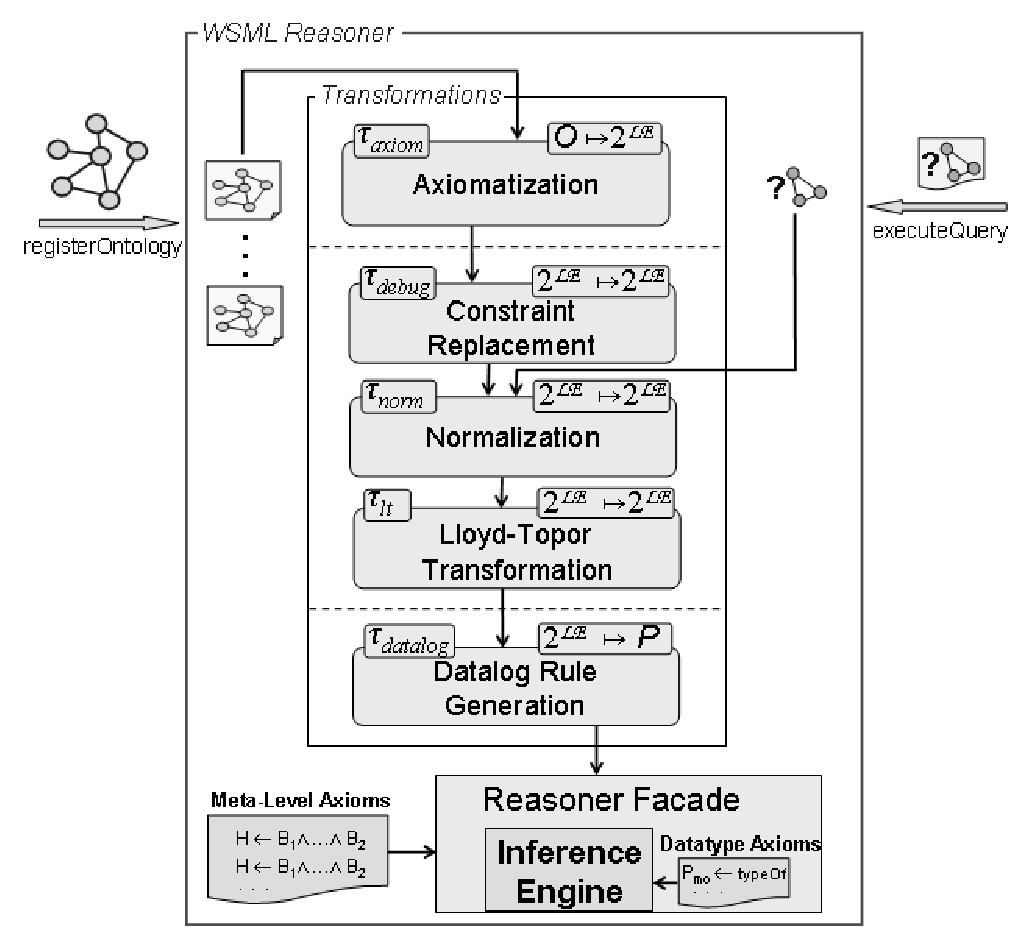
\includegraphics[width=11cm]{figures/layering}
    \centering
    \caption{Internal framework architecture. \label{fig:layering}}
\end{figure}
Figure~\ref{fig:layering} shows the internal architecture of the
framework as well as the data flow during a prototypical usage
scenario. The outer box outlines a WSML reasoner component that
allows a user to register WSML ontologies and to pose queries on
them. The inner box illustrates the transformation pipeline
introduced in Section \ref{sec:mapping} and shows its subsequent
steps in a layering scheme.

Registered ontologies go through all the transformation steps,
whereas user queries are injected at a later stage, skipping the
non-applicable axiomatization and constraint replacement steps.
Here, the internal layering scheme allows for an easy
reorganization and reuse of the transformation steps on demand,
assuring high flexibility and modularity. A good example for this
is the constraint replacement transformation \transdebug: if
included in the pipeline, it produces the rules that activate the
debugging features according to Section \ref{sec:debugging}; if
excluded, the constraints remain in the resulting Datalog program
and are mapped to native constraints of the underlying reasoning
engine.

The core component of the framework is an exchangeable Datalog
inference engine wrapped by a reasoner facade which embeds it in
the framework infrastructure. This facade mediates between the
generic Datalog program produced in the transformations and the
tool-specific Datalog implementation and built-in predicates used
by the external inference engine.

\subsection{Interface and Integration with Existing Technology}
So far we have not detailed on what data structure the framework
operates on. One could implement it directly with a parser and
compiler framework that generates an abstract syntax tree for WSML
which is then directly transformed to the target format (Datalog).
Although this would have performance advantages, it would greatly
reduce reusability and would make maintenance harder. Our framework
is based on an intermediate object model of the language that is
provided by the WSMO4J\footnote{\url{http://wsmo4j.sourceforge.net}}
project. WSMO4J performs the task of parsing and validating WSML
ontologies and provides the source object model for our
translations. In order to enable the usage of different Datalog
engines we additionally implemented a simple object model for
Datalog that is independent from any particular engine. The Datalog
model has objects to represent Literals and Rules, whereas the term
structure is directly reused from WSMO4J (respectively WSML). For
each reasoner that has to be connected to the Framework a small
adapter class has to be written, that is minimally aware of only
Literals, Rules and constants (IRIs) and has to translate them to
the equivalent within the representation of the reasoner. If a
particular reasoner supports additional built-ins and data types
translations for this can iteratively be added.

The WSML reasoner framework currently ships with Facades for two
built-in reasoners: KAON2 and MINS. The initial development was done
with the KAON2 inference engine\footnote{KAON2 is available for
download from \url{http://kaon2.semanticweb.org}}
\cite{hustadt04reducing}. As we have seen in
Section~\ref{sec:datatype_reasoning}, datatype reasoning poses the
biggest challenge for the Datalog implementation. KAON2 provides a
very flexible type system that allows for user-defined datatypes,
together with user-defined predicates on these datatypes, including
type checking predicates. Therefore, KAON2 meets the identified
requirements easily. As a matter of fact, KAON2 already provided
most of the required datatypes and predicates out of the box.

The second reasoner that is currently supported by the framework is
MINS\footnote{\url{http://dev1.deri.at/mins/}}. Whereas KAON2 is the
default reasoner for WSML Flight, MINS can be used for the WSML Rule
variant that includes function symbols and unsafe rules. For
determining which WSML variant a current ontology is in the user of
the framework can use the validation facilities built into
WSMO4J\footnote{A demo of this feature is available at:
\url{http://tools.deri.org/wsml/validator}}.

%\section{A Use Case Example for Reasoning with WSML Ontologies\label{sec:usecase}}
-- present a WSML example ontology that demonstrates the style of modelling in rule-based WSML, to give the reader an impression what he can do with the reasoning framework \\
\phantom{mm} -- -- how do constraints work \\
\phantom{mm} -- -- how do derivation rules work \\
\phantom{mm} -- -- how does debugging support ontology development \\
-- a candidate example is the WP8 telecom bundle scenario from the last DIP review \\

\section{Conclusion \& Outlook\vspace{-3mm}\label{sec:outlook}}
We have presented a framework for reasoning in rule-based WSML
that builds on a mapping to Datalog and on querying a generic
Datalog layer. The single well-defined transformation steps can be
reused across various adaptations for different scenarios in a
highly modular way. We have incorporated debugging features by
replacing native constraints with rules to derive
debugging-relevant information that can be queried by an ontology
engineer. We have implemented our framework with two existing
reasoner tools, namely KAON2 and MINS, as alternative
implementations of the generic Datalog layer, by which we provide
the first available reasoning system for the WSML language.

While the current framework focuses on WSML-Core, -Flight and
-Rule, efforts are ongoing to extend the transformations to
disjunctive Datalog and description logics. The KAON2 system
natively supports disjunctive Datalog and DL reasoning, the latter
even extended by WSML-Flight-like rules. Also the DLV
system~\cite{citrigno97dlv} (implementing disjunctive Datalog
under the stable model semantics) can be used to realise a similar
reasoning. Furthermore, we plan to integrate the KRHyper
system~\cite{wernhard03system}, which allows reasoning with
disjunctive logic programs with stratified default negation.
Transformations to DL additionally allow to incorporate
description logic system APIs to support efficient reasoning with
WSML-DL.


%\paragraph{Acknowledgements.}
%This work is supported by the European Commision under the DIP
%project (FP6-507483), and by the Austrian Federal Ministry for
%Transport, Innovation, and Technology under the project {\sffamily
% {\bfseries R}W$^{\mathsf{2}}$} (FFG 809250).


\bibliographystyle{plain}
\bibliography{paper}

}

\end{document}
